\begin{pastexam}[label={px:gw3-105-ds-02}]{關務三等資料處理 105 年 第二題}
（申論；35 分）

\begin{itemize}[leftmargin=2em, labelsep=0.3em, itemsep=2pt]
\item[㈠] 請解釋何謂引線二元樹（threaded binary tree）及其優點為何。（10 分）
\item[㈡] 若要以鏈結串列（linked list）來表達引線二元樹，試設計一適當之節點結構。（5 分）
\item[㈢] 請畫出下圖所示二元樹之引線二元樹。請分別畫出有頭端節點（header node）與無頭端節點之引線
二元樹。（10 分）
\begin{center}
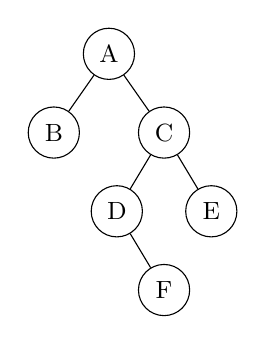
\begin{tikzpicture}[level distance=10mm,
  level 1/.style={sibling distance=14mm}, level 2/.style={sibling distance=12mm},
  every node/.style={circle, draw, minimum size=6.5mm, inner sep=0pt, font=\small}]
\node {A}
  child {node {B}}
  child {node {C}
    child {node {D} child[missing] child {node {F}}}
    child {node {E}}};
\end{tikzpicture}
\end{center}
\item[㈣] 請寫出在引線二元樹中以線性時間（即時間複雜度為 $O(n)$）進行中序尋訪的演算法。（10 分）
\end{itemize}
\end{pastexam}

\begin{pastsoln}
\textbf{㈠ 引線二元樹。} 用鏈結表示 $n$ 個節點的二元樹，$2n$ 個指標裡只有 $n - 1$ 個指向子節點，
其餘 $n + 1$ 個是空的（NULL）。 引線二元樹把這些空指標拿來用：
\begin{itemize}[nosep]
\item 左指標原本是空的，改成指向該節點在\textbf{中序}裡的前一個節點（前驅）；
\item 右指標原本是空的，改成指向中序裡的下一個節點（後繼）。
\end{itemize}
這些指標稱為\textbf{引線}（thread）；每個節點另外用兩個旗標區分指標是「子節點」還是「引線」
（資結書第~7.5~節）。
\textbf{優點}：
\begin{itemize}[nosep]
\item 中序走訪不需要堆疊也不需要遞迴，只用幾個變數，額外空間 $O(1)$（一般的中序走訪要 $O(h)$ 的
堆疊）。
\item 找任一節點的中序後繼（或前驅）很方便：右指標是引線就一步到位，不必從根重新找或存父節點指標。
\item 原本浪費的 $n + 1$ 個空指標被利用，每個節點只多兩個位元的旗標。
\end{itemize}
代價是插入、刪除時除了子節點指標，還要一併維護引線。

\textbf{㈡ 節點結構。}
\begin{center}
\begin{tabular}{|c|c|c|c|c|}
\hline
\texttt{lthread} & \texttt{left} & \texttt{data} & \texttt{right} & \texttt{rthread} \\ \hline
\end{tabular}
\end{center}
\begin{minted}[fontsize=\small, style=perldoc]{c}
#include <stdbool.h>

struct tnode {
    bool lthread;         /* true：left 是引線（指向中序前驅）；false：left 指向左子 */
    struct tnode *left;
    char data;
    struct tnode *right;
    bool rthread;         /* true：right 是引線（指向中序後繼）；false：right 指向右子 */
};
\end{minted}

\textbf{㈢} 先求中序：$B, A, D, F, C, E$。 原樹的空指標有 $7$ 個：$B$ 的左右、$D$ 的左、$F$ 的左右、
$E$ 的左右。 依中序的前後關係改成引線：
\begin{center}
\small
\begin{tabular}{cll}
\toprule
節點 & 左指標 & 右指標 \\
\midrule
$B$ & 引線 $\to$ 無前驅（NULL／頭端節點） & 引線 $\to A$ \\
$A$ & 子節點 $B$ & 子節點 $C$ \\
$D$ & 引線 $\to A$ & 子節點 $F$ \\
$F$ & 引線 $\to D$ & 引線 $\to C$ \\
$C$ & 子節點 $D$ & 子節點 $E$ \\
$E$ & 引線 $\to C$ & 引線 $\to$ 無後繼（NULL／頭端節點） \\
\bottomrule
\end{tabular}
\end{center}
下面實線是子節點指標，虛線箭頭是引線。

\textbf{無頭端節點}：中序第一個 $B$ 的左引線和最後一個 $E$ 的右引線沒有對象，設為 NULL（旗標仍為
true）。
\begin{center}
\begin{tikzpicture}[x=1.15cm, y=1.1cm, >=Stealth,
  v/.style={circle, draw, minimum size=6.5mm, inner sep=0pt, font=\small},
  th/.style={->, dashed, thin}]
\node[v] (A) at (0,0) {A};
\node[v] (B) at (-1.6,-1) {B};
\node[v] (C) at (1.6,-1) {C};
\node[v] (D) at (0.7,-2) {D};
\node[v] (E) at (2.5,-2) {E};
\node[v] (F) at (1.4,-3) {F};
\draw (A)--(B) (A)--(C) (C)--(D) (C)--(E) (D)--(F);
\node[font=\scriptsize] (n1) at (-2.6,-2) {NULL};
\node[font=\scriptsize] (n2) at (3.5,-3) {NULL};
\draw[th] (B) -- (n1);
\draw[th] (B) to[bend right=25] (A);
\draw[th] (D) to[bend left=25] (A);
\draw[th] (F) to[bend left=35] (D);
\draw[th] (F) to[bend right=40] (C);
\draw[th] (E) to[bend right=35] (C);
\draw[th] (E) -- (n2);
\end{tikzpicture}
\end{center}

\textbf{有頭端節點}：加一個不存資料的頭端節點 $H$。 $H$ 的 \texttt{left} 指向樹根 $A$（\texttt{lthread}
$=$ false），\texttt{right} 指向自己（\texttt{rthread} $=$ false）；原本是 NULL 的兩條引線（$B$ 的左、
$E$ 的右）都改指向 $H$。 這樣所有引線都有對象，走訪時從 $H$ 出發、回到 $H$ 就結束。 （空樹時
$H$ 的 \texttt{left} 指向自己、\texttt{lthread} $=$ true。）
\begin{center}
\begin{tikzpicture}[x=1.15cm, y=1.1cm, >=Stealth,
  v/.style={circle, draw, minimum size=6.5mm, inner sep=0pt, font=\small},
  th/.style={->, dashed, thin}]
\node[draw, rectangle, minimum width=9mm, minimum height=6mm, font=\small] (H) at (0,1.2) {H};
\node[v] (A) at (0,0) {A};
\node[v] (B) at (-1.6,-1) {B};
\node[v] (C) at (1.6,-1) {C};
\node[v] (D) at (0.7,-2) {D};
\node[v] (E) at (2.5,-2) {E};
\node[v] (F) at (1.4,-3) {F};
\draw (H)--(A);
\draw[->] (H.east) to[out=20, in=60, looseness=6] (H.north east);
\draw (A)--(B) (A)--(C) (C)--(D) (C)--(E) (D)--(F);
\draw[th] (B) to[out=150, in=180] (H);
\draw[th] (B) to[bend right=25] (A);
\draw[th] (D) to[bend left=25] (A);
\draw[th] (F) to[bend left=35] (D);
\draw[th] (F) to[bend right=40] (C);
\draw[th] (E) to[bend right=35] (C);
\draw[th] (E) to[out=30, in=0, looseness=1.2] (H);
\end{tikzpicture}
\end{center}
$H$ 上方的實線小圈是它指向自己的右指標，$H$ 到 $A$ 的實線是它的左指標。

\textbf{㈣ 中序走訪}（以有頭端節點的版本寫；無頭端節點時把「回到 $H$」換成「遇到 NULL」，見資結書
虛擬碼~7.6）。 中序後繼的找法：右指標是引線就直接是後繼；否則後繼是右子樹最左邊的節點。
\begin{pseudo}{引線二元樹的中序走訪（有頭端節點 $H$）}
\Function{In-Succ}{$x$}
    \State $y \gets x.\mathit{right}$
    \If{\textbf{not} $x.\mathit{rthread}$} \Comment{有右子樹：往右一步再一路往左}
        \While{\textbf{not} $y.\mathit{lthread}$}
            \State $y \gets y.\mathit{left}$
        \EndWhile
    \EndIf
    \State \Return $y$
\EndFunction
\Procedure{Threaded-Inorder}{$H$}
    \State $x \gets$ \Call{In-Succ}{$H$} \Comment{$H$ 的右子樹是整棵樹：得到中序第一個}
    \While{$x \ne H$}
        \State 拜訪 $x$
        \State $x \gets$ \Call{In-Succ}{$x$}
    \EndWhile
\EndProcedure
\end{pseudo}
這裡利用了 $H.\mathit{right} = H$、$H.\mathit{rthread} = \FALSE$ 的設定：\proc{In-Succ}($H$) 從
$H.\mathit{right} = H$ 開始往左走，經過 $A$ 一路走到中序第一個節點 $B$。

\textbf{追蹤}：\proc{In-Succ}($H$) 走 $H \to A \to B$（$B$ 的左邊是引線），拜訪 $B$；$B$ 的右引線 $\to A$；
$A$ 有右子樹，走 $C \to D$（$D$ 的左邊是引線），得 $D$；$D$ 有右子樹 $F$，$F$ 的左邊是引線，得 $F$；
$F$ 的右引線 $\to C$；$C$ 有右子樹 $E$，得 $E$；$E$ 的右引線 $\to H$，結束。 拜訪順序
$B, A, D, F, C, E$，正是中序。

\textbf{時間 $O(n)$}：每個節點被拜訪一次。 \proc{In-Succ} 裡往左走的步數加總起來，每一條「往左的
子節點邊」在整趟走訪中最多被走一次（每條左鏈只會從它頂端的父節點的右子出發走一次），所以總共不超過
$n$ 步；其餘每次呼叫是常數時間。 合計 $O(n)$，而且只用常數個變數，不需要堆疊。
\end{pastsoln}
